\subsubsection{Fungsionalitas pada Domain User}

Pengujian dengan ID P05 dilakukan dengan skenario yaitu admin berhasil membuat \textit{user} baru dengan nama, email, password, serta companyId yang valid. Admin akan membuat request dengan Postman kepada \textit{server} dengan request seperti berikut.

\begin{enumerate}
  \item Mengisi \textit{field name} dengan nilai "new user"
  \item Mengisi \textit{field email} dengan nilai "newuser@gmail.com"
  \item Mengisi \textit{field password} dengan nilai "inicontohpasswordges"
  \item Mengisi \textit{field company\textunderscore id} dengan nilai "d6c03902-3758-47bd-994d-616e1917cc61"
\end{enumerate}

\textit{Request} dibuat dengan membuat request menggunakan Postman pada url /admin-api/v1/users dengan metode POST. \textit{Request dan response} dapat dilihat pada gambar \ref{fig:pengujian-p05}

\begin{figure}[ht]
  \centering
  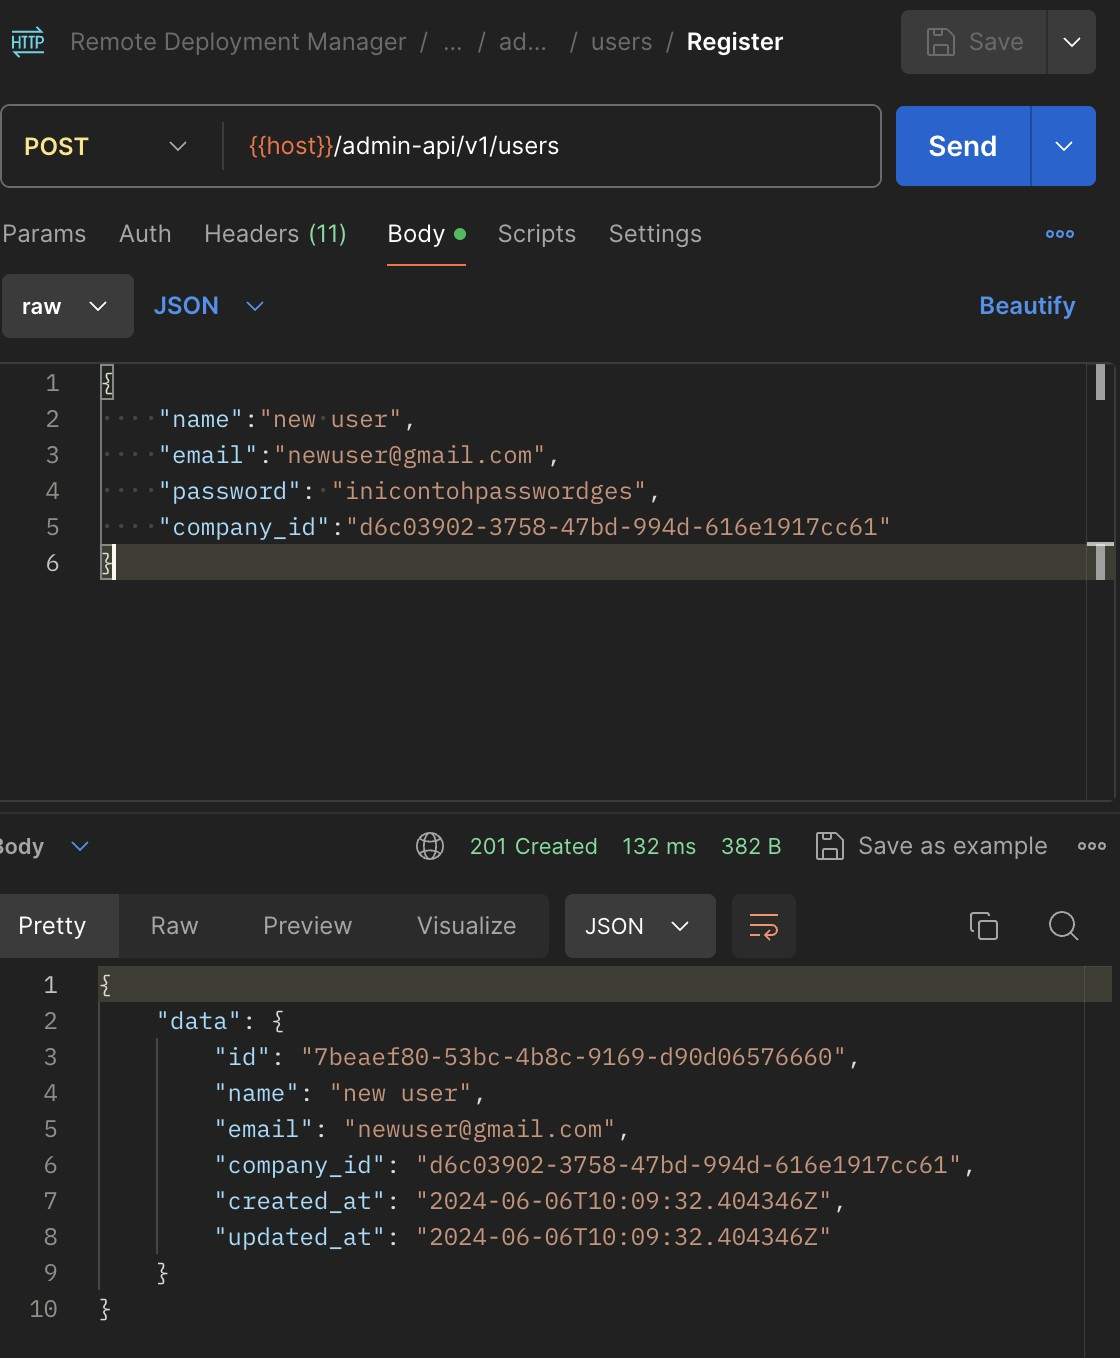
\includegraphics[width=0.8\textwidth]{resources/chapter-4/pengujian/p05.jpg}
  \caption{\textit{Request dan Response Pengujian} P05}
  \label{fig:pengujian-p05}
\end{figure}

% Pengujian dengan ID P02 dilakukan dengan skenario yaitu admin tidak berhasil membuat \textit{user} karena nama cluster yang tidak tersedia pada server. Tersedia berarti, konfigurasi kubernetes cluster terdapat pada kubernetes \textit{config server} Admin akan membuat request dengan Postman kepada server dengan request seperti berikut.

% \begin{enumerate}
%   \item Mengisi \textit{field name} dengan nilai "new user"
%   \item Mengisi \textit{field cluster\textunderscore name} dengan nilai "kind-psa-with-cluster-ps"
% \end{enumerate}

% \textit{Request} dibuat dengan membuat request menggunakan Postman pada url /admin-api/v1/companies dengan metode POST. \textit{request dan response} dapat dilihat pada gambar

% \begin{figure}[ht]
%   \centering
%   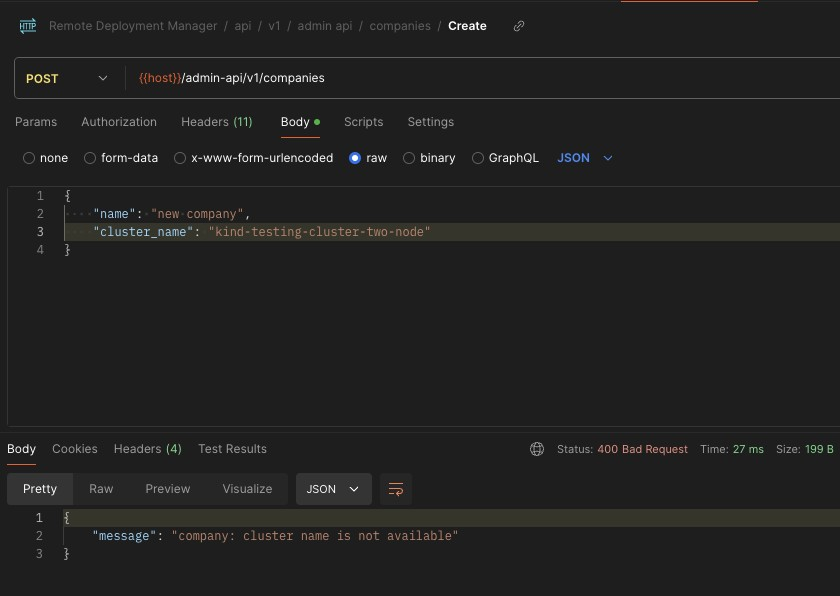
\includegraphics[width=0.8\textwidth]{resources/chapter-4/pengujian/p02.jpg}
%   \caption{\textit{Request dan Response Pengujian} P02}
%   \label{fig:pengujian-p02}
% \end{figure}

% Pengujian dengan ID P03 dilakukan dengan skenario yaitu admin ingin mendapatkan seluruh \textit{user} yang terdaftar pada sistem. Admin akan membuat GET request dengan Postman ke url /admin-api/v1/companies. Berikut merupakan balikan dari \textit{request} yang dikirimkan

% \begin{figure}[ht]
%   \centering
%   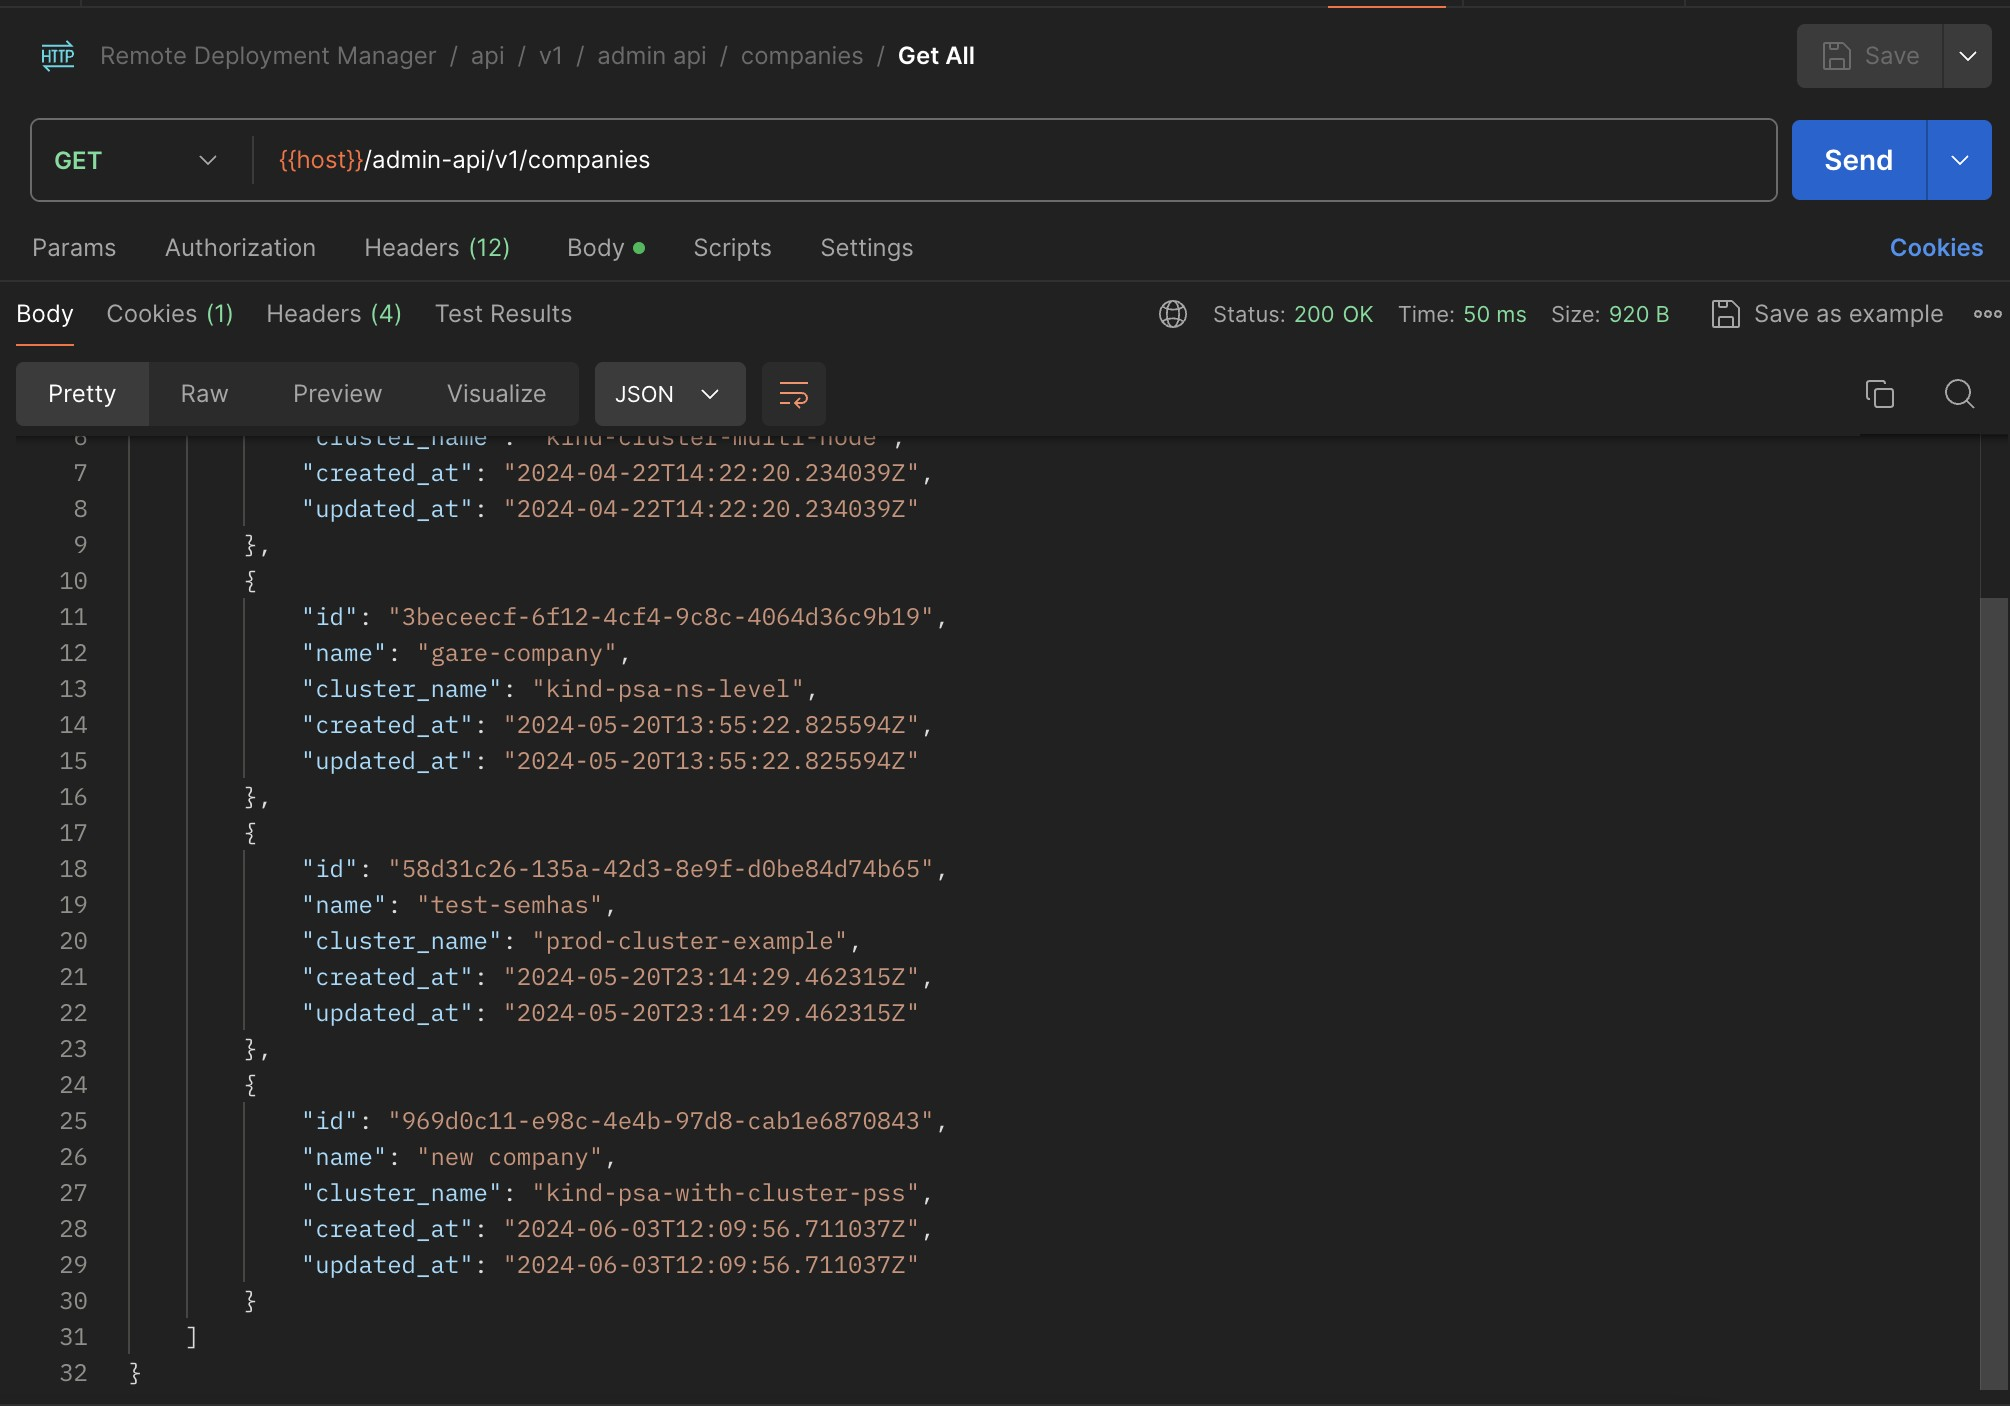
\includegraphics[width=0.8\textwidth]{resources/chapter-4/pengujian/p03.jpg}
%   \caption{\textit{Request dan Response Pengujian} P03}
%   \label{fig:pengujian-p03}
% \end{figure}

% Pengujian dengan ID P04 dilakukan dengan skenario yaitu admin ingin menghapus \textit{user} dengan id tertentu dari daftar \textit{user} pada sistem. Admin akan membuat DELETE request dengan Postman ke url /admin-api/v1/companies/:id. Admin menggunakan id user yang berhasil dibuat sesuai dengan gambar \ref{fig:pengujian-p01} sebagai parameter untuk \textit{user} yang dihapus. Berikut merupakan balikan dari \textit{request} yang dikirimkan.

% \begin{figure}[ht]
%   \centering
%   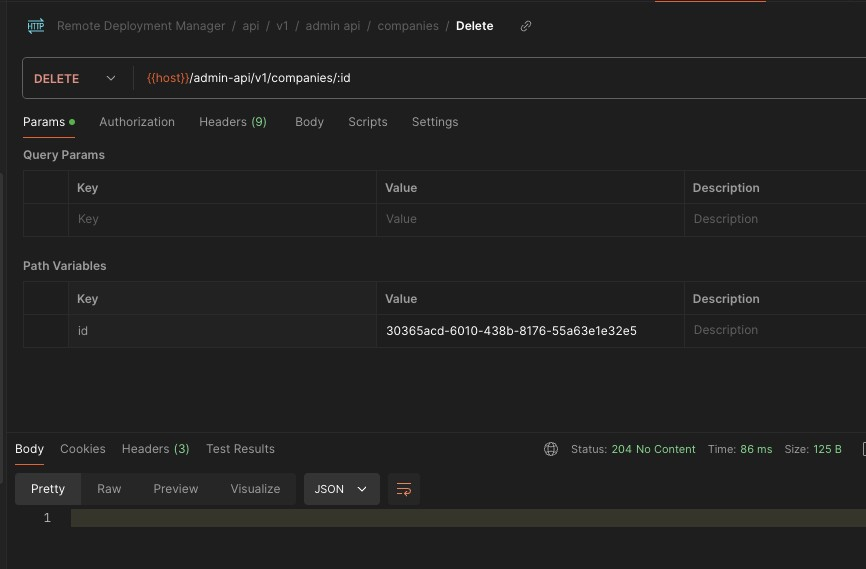
\includegraphics[width=0.8\textwidth]{resources/chapter-4/pengujian/p04.jpg}
%   \caption{\textit{Request dan Response Pengujian} P04}
%   \label{fig:pengujian-p04}
% \end{figure}

% Seluruh rekap pengujian pada domain \textit{user} dapat dilihat pada tabel \ref{tab:pengujian-domain-user}. Berdasarkan hasil yang diperoleh, terbukti bahwa kebutuhan fungsional dengan ID F01, F02, dan F03 telah terimplementasi dengan baik.


% \bgroup
% \begin{table}[ht]
%   \def\arraystretch{1.5}
%   \caption{Skenario dan Hasil Pengujian Domain \textit{Company}}
%   \label{tab:pengujian-domain-user}
%   \centering
%   \begin{tabular}{|p{2cm}|p{2cm}|p{4cm}|p{3cm}|p{2cm}|}
%     \hline
%     \centering{ID Fungsional} & \centering{ID Pengujian} & \centering{Skenario}                                                              & \centering{Ekspektasi}                                                                       & Realita \\
%     \hline
%     F01                       & P01                      & Admin mendaftarkan \textit{user} dengan cluster name yang tersedia                & Admin berhasil mendaftarkan \textit{user}                                                    & Sesuai  \\
%     \hline
%     F01                       & P02                      & Admin mendaftarkan \textit{user} dengan cluster name yang tidak valid             & Admin tidak berhasil mendaftarkan karena cluster name tidak valid                            & Sesuai  \\
%     \hline
%     F02                       & P03                      & Admin membuat \textit{request} untuk melihat seluruh \textit{user} pada sistem    & Admin dapat melihat seluruh \textit{user} pada sistem                                        & Sesuai  \\
%     \hline
%     F03                       & P04                      & Admin melakukan DELETE \textit{request} untuk menghapus \textit{user} pada sistem & Admin dapat menghapus \textit{user} pada sistem dengan memberikan id user yang ingin dihapus & Sesuai  \\
%     \hline
%   \end{tabular}
% \end{table}
% \egroup


